\documentclass[12pt]{article}
\usepackage{graphicx}
\usepackage{graphics}
\usepackage{amssymb}
\usepackage{hyperref}
\usepackage{multirow}
\usepackage{amsmath}
\usepackage{tabularx}
\usepackage{float}

\title{Final Report: Rate My Teammate (ver.CWRU)}
\author{Haihan Jiang, Liyuan Huang, Nora Tang, Walter Nam \footnote{All are from Department of Computer Science.}}
\date{November 2021}
\begin{document}
\maketitle
\begin{abstract}
    Rate My Teammate (version CWRU) is a web-application for Case Western Reserve University students who wish to find partners for course projects or competitions. We are aware CWRU students who want to collaborate on projects or competitions tend to find collaborative teammates who have expected skills or capability. 
We also conducted thorough competitor analysis on strengths and weaknesses of similar websites to facilitate our design procedures. A popular website among college students called “Rate My Professor” helps students pick the classes with the best professors based on user reviews. It contains a user-friendly interface, but does not easily filter departments by specific criteria. Therefore, the main functions of this project focus on an intuitive user interface, rating and reviewing teammates, and displaying necessary information of the student while preserving their privacy. Thus, the major functionalities include Signup, Login, Search by CaseID/Name/Majors which serves as a filter, Add New Students, Add New Reviews, Submit Review Corrections, Display Searching Results, and Display Rating Summary. To encourage data heterogeneity of the website, some constraints, such as students can only add new reviews if they already logged in or signed up, are enforced. The project is developed with SpringBoot as back-end, React.js as front-end, MySQL as database management. When fully developed, CWRU students will be able to use their CaseIDs to register and utilize the above mentioned functionalities. 

\end{abstract}
\section{Introduction}

	Colleges offer many project-based courses. Some of these projects need multiple students to collaborate on a project. Therefore, some students may encounter partners who are not suitable for their collaborations. For example, they may not have a  matched tech stack or they do not have enough time for collaborations. These factors may all contribute to an unsuccessful collaboration.  
To address this problem, we want to build a website application that can help Case Western Reserve University students to filter information on other students with clear rating criterias. We analyze other competitors in the market, RateMyProfessor and RateMyDorm, to learn lessons about the design. In the later sections of this report, we will show our competitor analysis and functionalities to show the strength of our product. 

\section{Competitor Analysis}
Based on the user's needs, we can see that students who want to collaborate 
on projects or competitions tend to hope to find their teammates effectively 
and efficiently. Therefore, we try to find three functionalities(Information 
Filter, Rating \& Review, Information’s Display) in our competitors: 
Rate My Professor and Rate My Dorm to analyze their weakness and strengths 
for concluding our core functionalities.
\subsection{Main Function1: Information Filter}

\begin{enumerate}
    \item \textbf{Rate My Professor: }
    
    \textbf{Strength: }

    \begin{itemize}
        \item The search bar is placed at a center place, and users can use the search function, which is a core function for Rate my Professor.
        \item It can filter by two key features: School and Professors, or combine two key features together.
    \end{itemize}
    \textbf{Weakness: }
    \begin{itemize}
        \item It cannot filter with courses (students may want to compare the rating between different professors who taught the same course).
        \item It cannot directly choose from students who take the same course.
    \end{itemize}
    \item \textbf{Rate My Dorm: }
    
    \textbf{Strength: }
    \begin{itemize}
        \item It has a clear and distinctive feature filter for quick locating information.
        \item Its sorting function enables users access to targeted objects in a short time.
    \end{itemize}
    \textbf{Weakness: }
    \begin{itemize}
        \item There is no clear tag in reviews, so users will find it hard to extract information from reviews.
        \item Types of Filters are very general and not very intuitive for users.
\end{itemize}
\end{enumerate}

\subsection{Main Function 2: Rating and Review}

\begin{enumerate}
    \item \textbf{Rate My Professor: }
    
    \textbf{Strength: }

    \begin{itemize}
        \item It has appropriate rating criteria for users to clearly see the instructor’s capability of teaching.
        \item It has specific review tags for users to efficiently select the instructor’s teaching style. 
    \end{itemize}
    \textbf{Weakness: }
    \begin{itemize}
        \item There is no way to verify the user, many fake accounts have been made to generate fake information about professors.
    \end{itemize}
    \item \textbf{Rate My Dorm: }
    
    \textbf{Strength: }
    \begin{itemize}
        \item It has several essential rating (bedroom, bathroom,...) breakdown.
        \item It displays useful reviewer info.
    \end{itemize}
    \textbf{Weakness: }
    \begin{itemize}
        \item It does not have review guidelines.
\end{itemize}
\end{enumerate}


\subsection{Main Function3: Information’s Display}

\begin{enumerate}
    \item \textbf{Rate My Professor: }
    
    \textbf{Strength: }

    \begin{itemize}
        \item It has clear yes/no for essential questions.
        \item It has clear and useful tag display (like top tags).
    \end{itemize}
    \textbf{Weakness: }
    \begin{itemize}
        \item It cannot update with the student’s improvement
    \end{itemize}

    \item \textbf{Rate My Dorm: }
    \textbf{Strength: }
    \begin{itemize}
        \item It has clear class breakdown.
    \end{itemize}
    \textbf{Weakness: }
    \begin{itemize}
        \item It does not include some important information (such as location, price).
\end{itemize}
\end{enumerate}

\section{Design Goal}
The design goal of our project is shown in Table~\ref{designgoal}.
\begin{table}[!htbp]
    \label{designgoal}
    \resizebox{\textwidth}{!}{%
    \begin{tabular}{|l|l|l|}
    \hline
    Objective         & Success Criteria                                                                                                                                                                                                                                                                                                                                                                                                                                                                                                                                                       & \multicolumn{1}{c|}{Status} \\ \hline
    Signup            & \begin{tabular}[c]{@{}l@{}}The user should be able to sign up by \\ inputting required information.\end{tabular}                                                                                                                                                                                                                                                                                                                                                                                                                                                       & complete                    \\ \hline
    Login             & \begin{tabular}[c]{@{}l@{}}The existent user should be able to login \\ with the correct caseID and password.\end{tabular}                                                                                                                                                                                                                                                                                                                                                                                                                                             & complete                    \\ \hline
    Add new student   & \begin{tabular}[c]{@{}l@{}}The logged-in user should be able to see and click on the \\ add new student button at the bottom of the search result page.\\ The user then should be able to add new student by \\ inputting required information.\\ The user who does not login should not be able to \\ see the button and should not be able to access the page.\end{tabular}                                                                                                                                                                                          & complete                    \\ \hline
    Add new review    & \begin{tabular}[c]{@{}l@{}}The logged-in user should be able to see and click on the add new review button \\ at the bottom of the student page.\\ The user then should be able to add new review \\ by inputting required information.\\ The user could review the same student only once.\\ The user who does not login should not be able to see the button and \\ should not be able to access the page.\end{tabular}                                                                                                                                              & complete                    \\ \hline
    Submit correction & \begin{tabular}[c]{@{}l@{}}The logged-in user should be able to see and click on the \\ submit correction button at the bottom left of each review \\ shown on the student page.\\ The submit correction page should be able to display \\ information of the previous review.\\ The user then should be able to submit correction by inputting \\ required information.\\ The user could submit correction only for his/her own review.\\ The user who does not login should not be able to see the button and \\ should not be able to access the page.\end{tabular} & complete                    \\ \hline
    Search main page  & \begin{tabular}[c]{@{}l@{}}The user should be able to input the text in the search bar. \\ And the user should be able to interact with the search button.\end{tabular}                                                                                                                                                                                                                                                                                                                                                                                                & complete                    \\ \hline
    Search result     & \begin{tabular}[c]{@{}l@{}}The user should be able to see the search result of \\ input information of the search bar.\end{tabular}                                                                                                                                                                                                                                                                                                                                                                                                                                    & complete                    \\ \hline
    Student page      & The user should be able to see the reviews of certain student.                                                                                                                                                                                                                                                                                                                                                                                                                                                                                                         & complete                    \\ \hline
    Navigation Bar    & \begin{tabular}[c]{@{}l@{}}The user who does not login should be able to see the signup/login\\  button on the top right of each page.\\ The logged-in user should be able to see the logout button \\ on the top right of each page.\\ The user should be able to see the rate my teammate icon \\ on the top left of each page except the main search page.\end{tabular}                                                                                                                                                                                             & complete                    \\ \hline
    \end{tabular}%
    }
    \caption{The design goal and success criteria of the project.}
    \end{table}


\section{Implementation}
\subsection{Backend}

\subsubsection {Database}
In database implementation, we planned to store user data in a server. The database should contain 8 entities and 7 relationships among them. In our design, we implemented on-to-one and one-to-many relationships based on our design goals. 
The ER diagram of database is designed as as Figure \ref{fig:er}.

\subsubsection {Data Manipulation}
For data manipulation, we used maven to insert depenencies we need. In this project, we used JDBC river,Hibernate, and Spring Data JPA. After all setups are done, wee are able to build entites classes an encapsulate them with clear annotations, which are used to map between database and our maven project. Then we created JPA repositories to use some inbuilt methods to implement CRUD(create, read, update, and delete) operations. Also, we added some JPQL queries mapping to SQL queries in our database. In this way, we could manipulate our data easily.

\subsubsection {Controllers}
For controllers, we implement logic code in different controllers for logic control. We called different Service instances to implement our functionalities: they include Sign up, Sign in, Update Review, Update Profile, Review Correction, and Profile Correction. At the same time, we provided RESTful API to collaborate with front-end subteam.

\begin{figure}[htp]
    \centering
    \label{fig:er}
    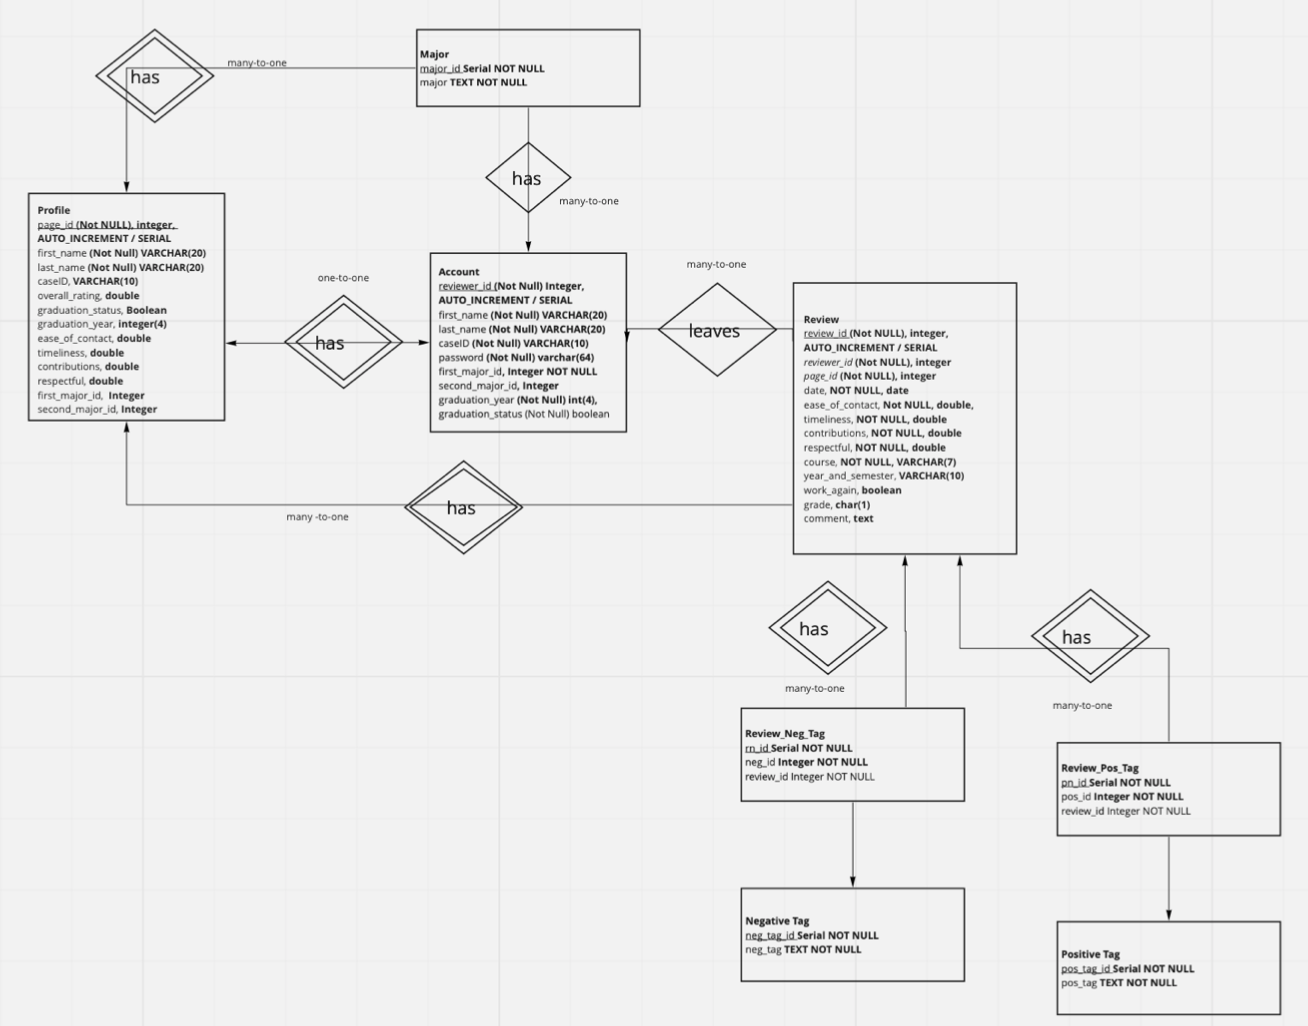
\includegraphics[scale=0.48]{er.png}
    \caption{The ER-diagram design of the database.}
\end{figure}

\subsection{Front-end}
We noticed that some pages share the same components. For example, signup page and add new student page both have 
first name, last name, caseID, and graduation year text fields.
To facilitate our design, we first broke down the components of each page and 
the map is shown in Figure \ref{fig:frontend}.
\begin{figure}[h]
    \centering
    \label{fig:frontend}
    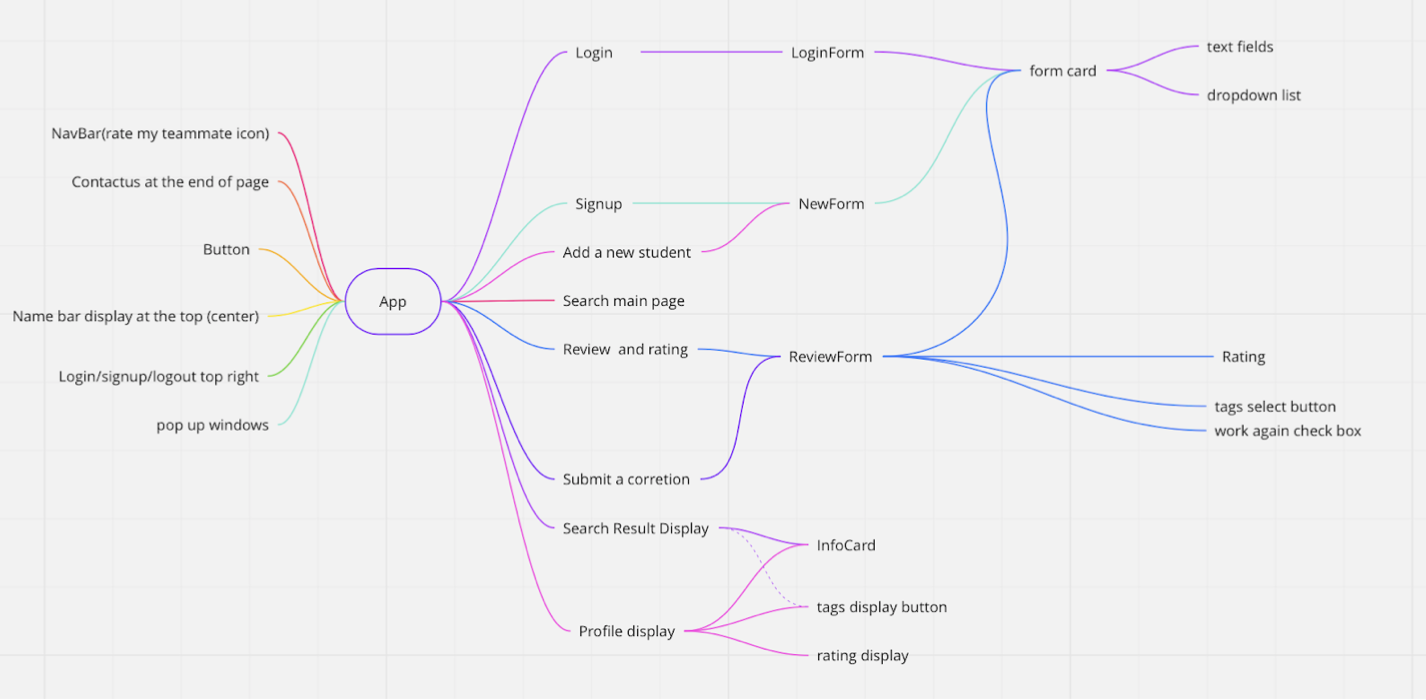
\includegraphics[scale=0.5]{front-end.png}
    \caption{The component breakdown of the front-end.}
\end{figure}
Then the front-end is built upon the above map as shown in Figure~\ref{fig:str}. 

\begin{figure}[h]
    \centering
    \label{fig:str}
    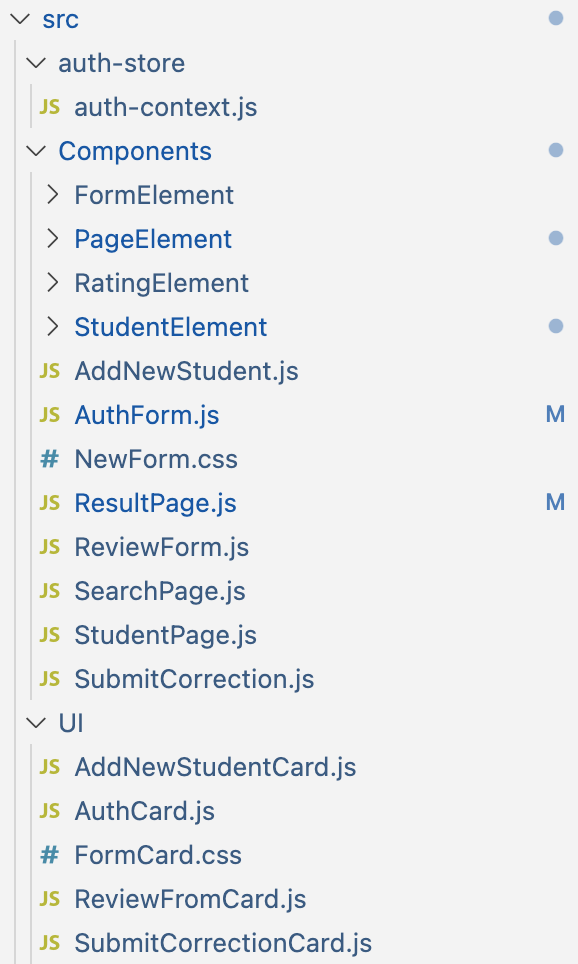
\includegraphics[scale=0.5]{front-str.png}
    \caption{The structure of the front-end.}
\end{figure}
In the \textit{auth-store} folder, 
we stored the status of the user (login or logout) because for some pages such as add new student, and add new review, 
only logged-in users are able to utilize these functionalities. The status will also be automatically reset, i.e., users 
will be automatically logged out, after one hour.

In the \textit{Components} folder, we have several element folders for the use of different pages. \textit{FormElement} contains 
necessary components of our form pages, including caseID, password, majors, etc. \textit{PageElement} contains elements designed 
for main page and navbar including search bar, search button, etc.  \textit{RatingElement} contains essential parts of rating forms 
including rating of several metrics, comment text field, tags, etc. \textit{StudentElement} includes components of 
profile page, including add new review button, reviews of the student, etc.

Here, we do not intend to go through the detailed design of each page, but we would like to present two examples to provide an overview in the following parts 
\footnote{For more details, please refer to \ref{repo}}. 
\subsubsection{AuthForm}
Rather than designing two different pages for login and signup, it would be much more efficient to combine the two forms into one by storing 
the user's certain action as a trigger of the switch. As shown in Figure~\ref{fig:authf}, \textit{isLogin} will store the trigger of the user, 
if it's false, then the page will display necessary text fields for signup, otherwise it will only display caseID and password.

\begin{figure}[h]
    \centering
    \label{fig:authf}
    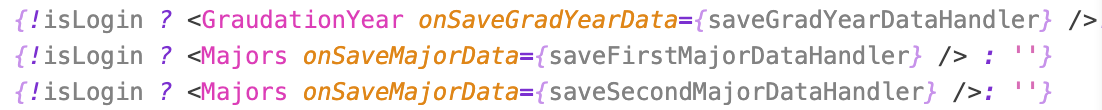
\includegraphics[scale=0.6]{auth-form.png}
    \caption{Code snapshot of the authorization form.}
\end{figure}

\subsubsection{ReviewForm}
One of the most important functionality of the review form is to provide users selection of tags. 
Figure~\ref{fig:tagren} shows the negative tag rendering in the review form. Users could select and de-select 
the tags, and the result of interaction will be recorded through \textit{saveNegTagDataHandler} and \textit{removeNegTagDataHandler}. 
The former one stores the IDs of selected tags as a list. The tricky part happens when users try to de-select some tags. 
Whenever such action occurs, \textit{removeNegTagDataHandler} will first detect the ID of the de-selected tag, and then filter the saved 
tag ID list to renew and store the latest tags as shown in Figure~\ref{fig:remtag}.
\begin{figure}[h]
    \centering
    \label{fig:tagren}
    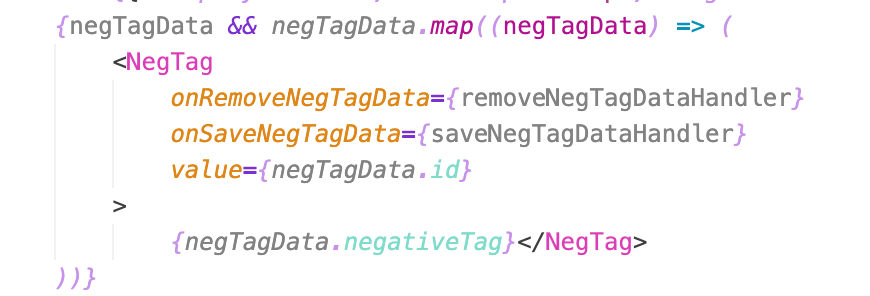
\includegraphics[scale=0.6]{tag-render.png}
    \caption{Code snapshot of the review form regarding the tag rendering.}
\end{figure}

\begin{figure}[h]
    \centering
    \label{fig:remtag}
    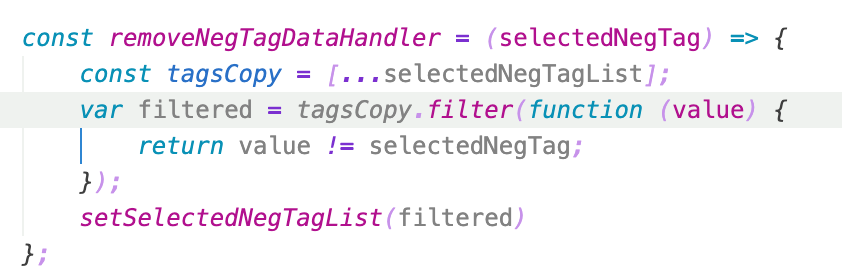
\includegraphics[scale=0.6]{remove-tag.png}
    \caption{Code snapshot of the review form regarding the remove tag functions.}
\end{figure}

\section{Overall Functionality}
\subsection{Search by CaseID/Major/Name}
The user could search for students by caseID, major, and name as shown in Figure~\ref{fig:search}.

\textbf{Status: Complete}

\subsection{Display Search Result}
The website will display search result of users' input which will include the average ratings, course, graduation year and so on of each student 
as shown in Figure~\ref{fig:result}.

\textbf{Status: Complete}

\subsection{Login/Signup}
Users can sign up and automatically create their own profile by filling in the authorization form as shown in Figure~\ref{fig:signup}. 
User can also log in using caseID and password as shown in Figure~\ref{fig:login}. 

\textbf{Status: Complete}

\subsection{Add a New Student}
Users who have logged in can add a student who doesn't have a profile yet to the website as shown in Figure~\ref{fig:add}.

\textbf{Status: Complete}

\subsection{Add a New Review}
Users who have logged in can add a new review for a student if they haven't reviewed yet as shown in Figure~\ref{fig:review}.

\textbf{Status: Complete}

\subsection{Submit Review Correction}
Users who are the authors of the review can submit correction of the review as update as shown in Figure~\ref{fig:correction}.

\textbf{Status: Complete}

\subsection{Display Student Page}
The comments and information display is one of the most essential parts of the application. 
Users are able to see the ratings, past comments, and related information 
(such as majors, project courses, graduation year) of the specific student as shown in Figure~\ref{fig:profile}

\textbf{Status: Complete}

\section{Discussion}

The information displayed demonstrates the integration of both the frontend and backend elements. The backend controllers are logically linked to the database functions and use RESTful API to connect to the frontend. Additionally, with the JDBC driver and Spring Data JPA, entities classes were developed along with annotations to map the SQL database with the backend maven project. As such, the overall functionalities listed above are linked to the frontend react components and are controlled by the logic mappings via JDBC and Spring Data JPA as specified in the Project Object Manager. The coverage reports from the testing of the integrated backend entities and controllers are supplemented below, demonstrating sufficient coverage.
\begin{center}
    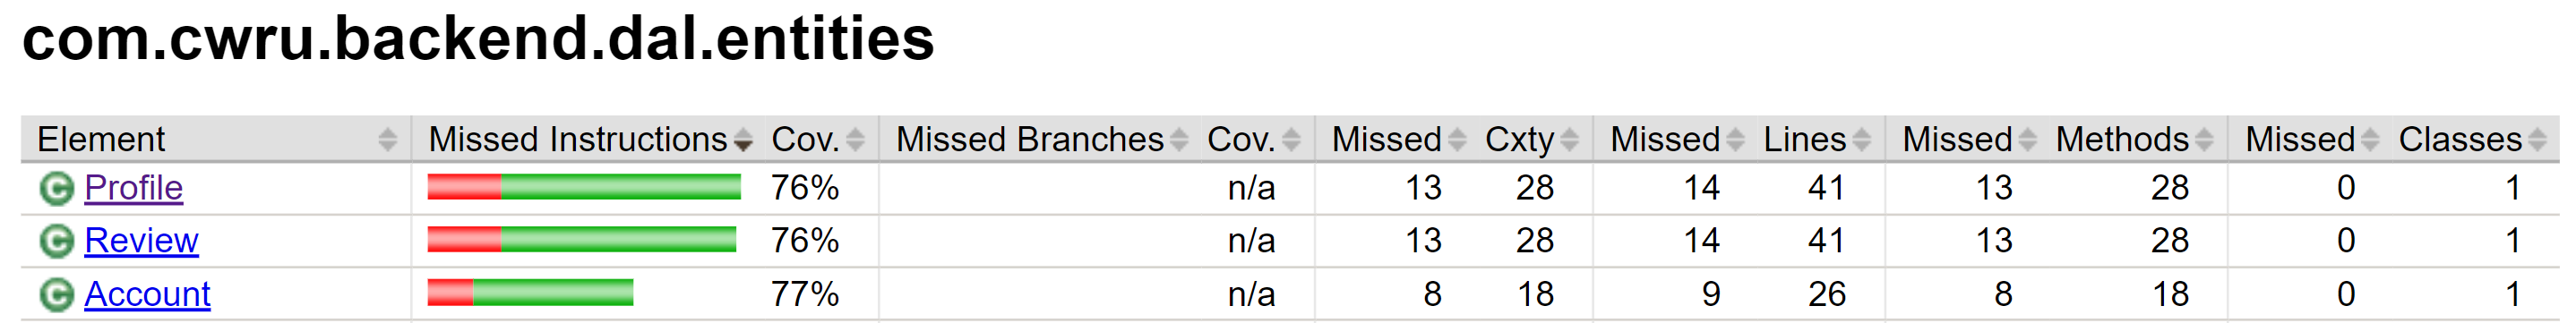
\includegraphics[scale = 0.3]{first.png}
\end{center}
\begin{center}
    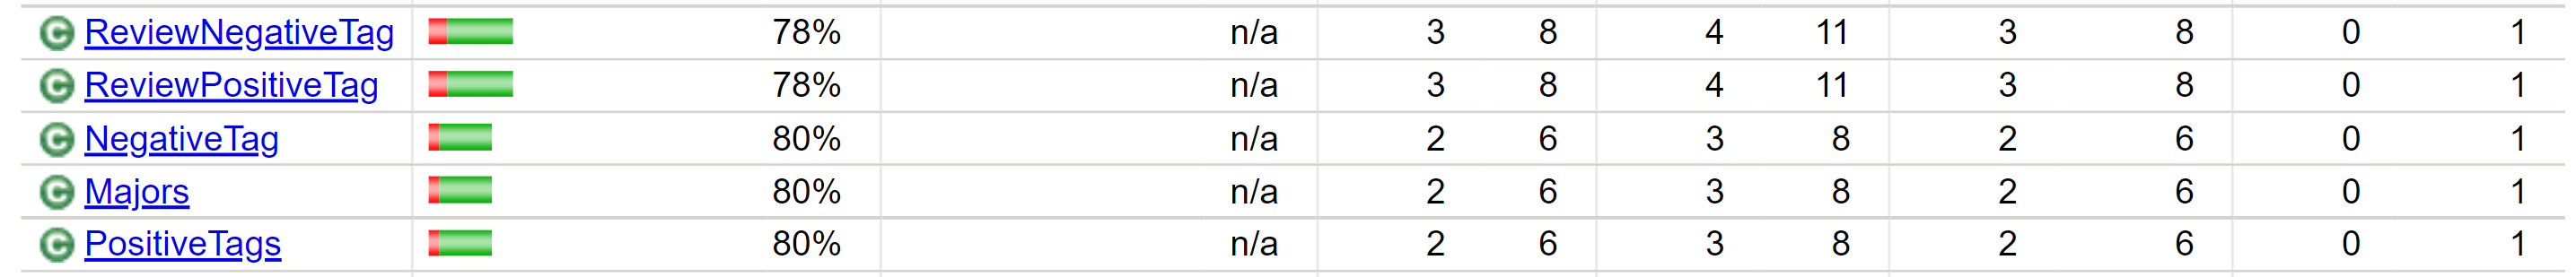
\includegraphics[scale = 0.3]{second.png}
\end{center}


\section{Work Allocation}
\begin{itemize}
    \item \textbf{Nora Tang: } 
    \\1. Participated in the design and implementation of the database.
    
    2. As a member of front-end sub-team, implemented code in the \textbf{/FormElement}, 
    \textbf{/RatingElement}, and \textbf{/StudentElement} (UI)folders, 
    \textbf{AuthForm.js}, \textbf{AddNewStudent.js}, \textbf{ReviewForm.js}, 
    \textbf{StudentPage.js} (UI), \textbf{SubmitCorrection.js}, and configured the initial routing for each page. 
    
    3. Wrote \textbf{ReviewNegativeTagsController.java, ReviewPositiveTagsController.java, NegativeTagController.java, PositiveTagController.java.}, 
    and \textbf{Review/add}, \textbf{Review/update} of ReviewController.java of the backend. 
    
    4. Participated in writing API document for REST API.
    
    5. Fixed minor bugs in the back-end code.
    
    \item \textbf{Liyuan Huang: }
    \\ 1. Participated in the design and implementation of the database.
    
    2. As a member of front-end sub-team, implemented result page, navigation bar, website icon, and card wrappers under the /UI folder. Participated in the implementation of search page. Also completed the connection between search, result, student pages with the back-end, and the data parameters passing between search, result, student, review, and submit correction pages. 
    
    3. Created and wrote the API document for REST API.
    
    4. Fixed minor bugs in the back-end code.
    
    \item \textbf{Haihan Jiang: }
    \\1.Maven Configurations for dependencies with JDBC drive and Spring JPA Data.

	2.Completed \textbf{Every Model Class} mapping to MySQL Database tables.

	3.Completed \textbf{Every Repository Interface} with JPA repositories to ensure basic CRUD(Create,Read,Update,Delete) operation and customized Criteria Search.

	4.Completed \textbf {Every Service Interface and Service Implementation Class}.

	5.Completed \textbf {Account,Major,Profile,Review Controllers} in backend to guarantee SignUp, Login, Search, Update Profile, Review Correction functionalities could work peoperly.
    \item \textbf{Walter Nam: }
    \\1. Participated in the UI design and functionality of the web application.
    
      2. Participated in the design and development of the database, including the ER diagram and sample queries. 
    
      3. Set up the template code for the backend maven project, ensured the correct project structuring and hierarchy.
    
      4. Generated coverage report using JaCoCo on build to ensure code entities were properly functioning. 
\end{itemize}

\section{Conclusion}
The final product of the Rate My Teammate web application meets most of our expectations in the proposal report. With our cooperation and hard work through this semester, we implemented features that include Sign up, Log in, search by Major/CaseID/name, Add a new student, add a new review in perspective of rating, class information, and comments, and submit a correction for the review. In general, our web application exhibits a high level of usefulness -- help Case students to have a general idea about classmates' personalities and capabilities, and find teammates who have expected skills to complete projects or competitions.

\section{Appendix}
\subsection{GitHub Repository}
\label{repo}
Please refer to \href{https://github.com/jyyy03/CSDS395_Rate_My_Teammate}{this link} for more implementation details.
\subsection{Front-end Snapshots}
\begin{figure}[h]
    \centering
    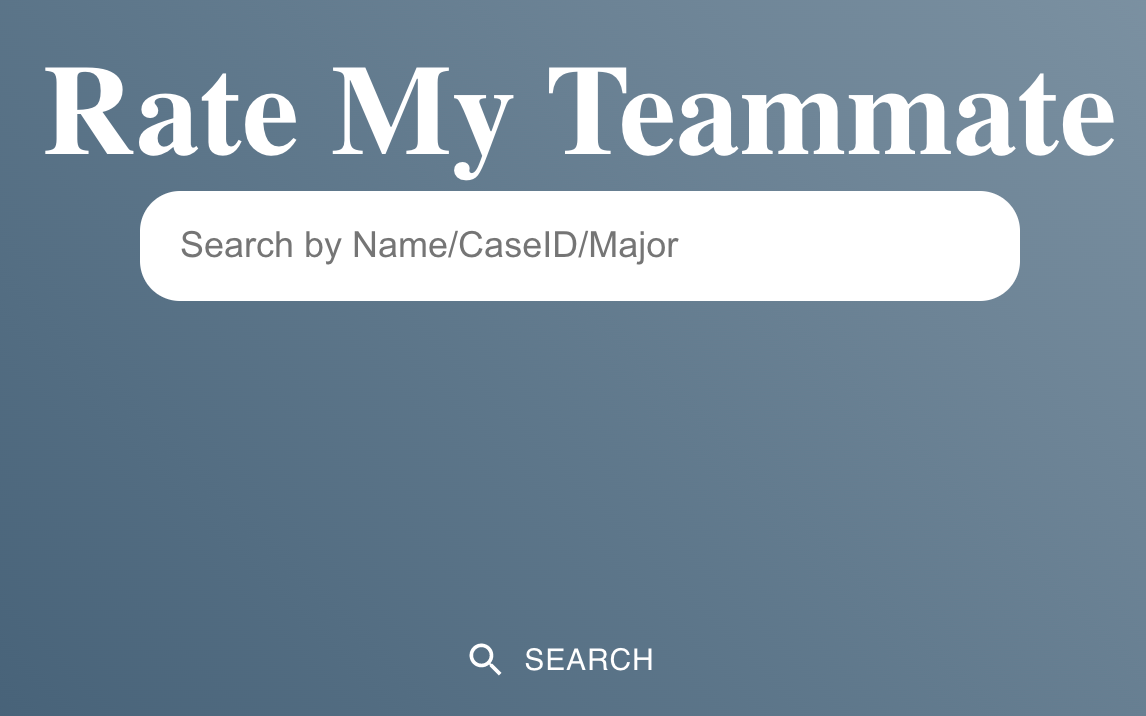
\includegraphics[scale=0.6]{search.png}
    \caption{Search Page}
    \label{fig:search}
\end{figure}

\begin{figure}[h]
    \centering
    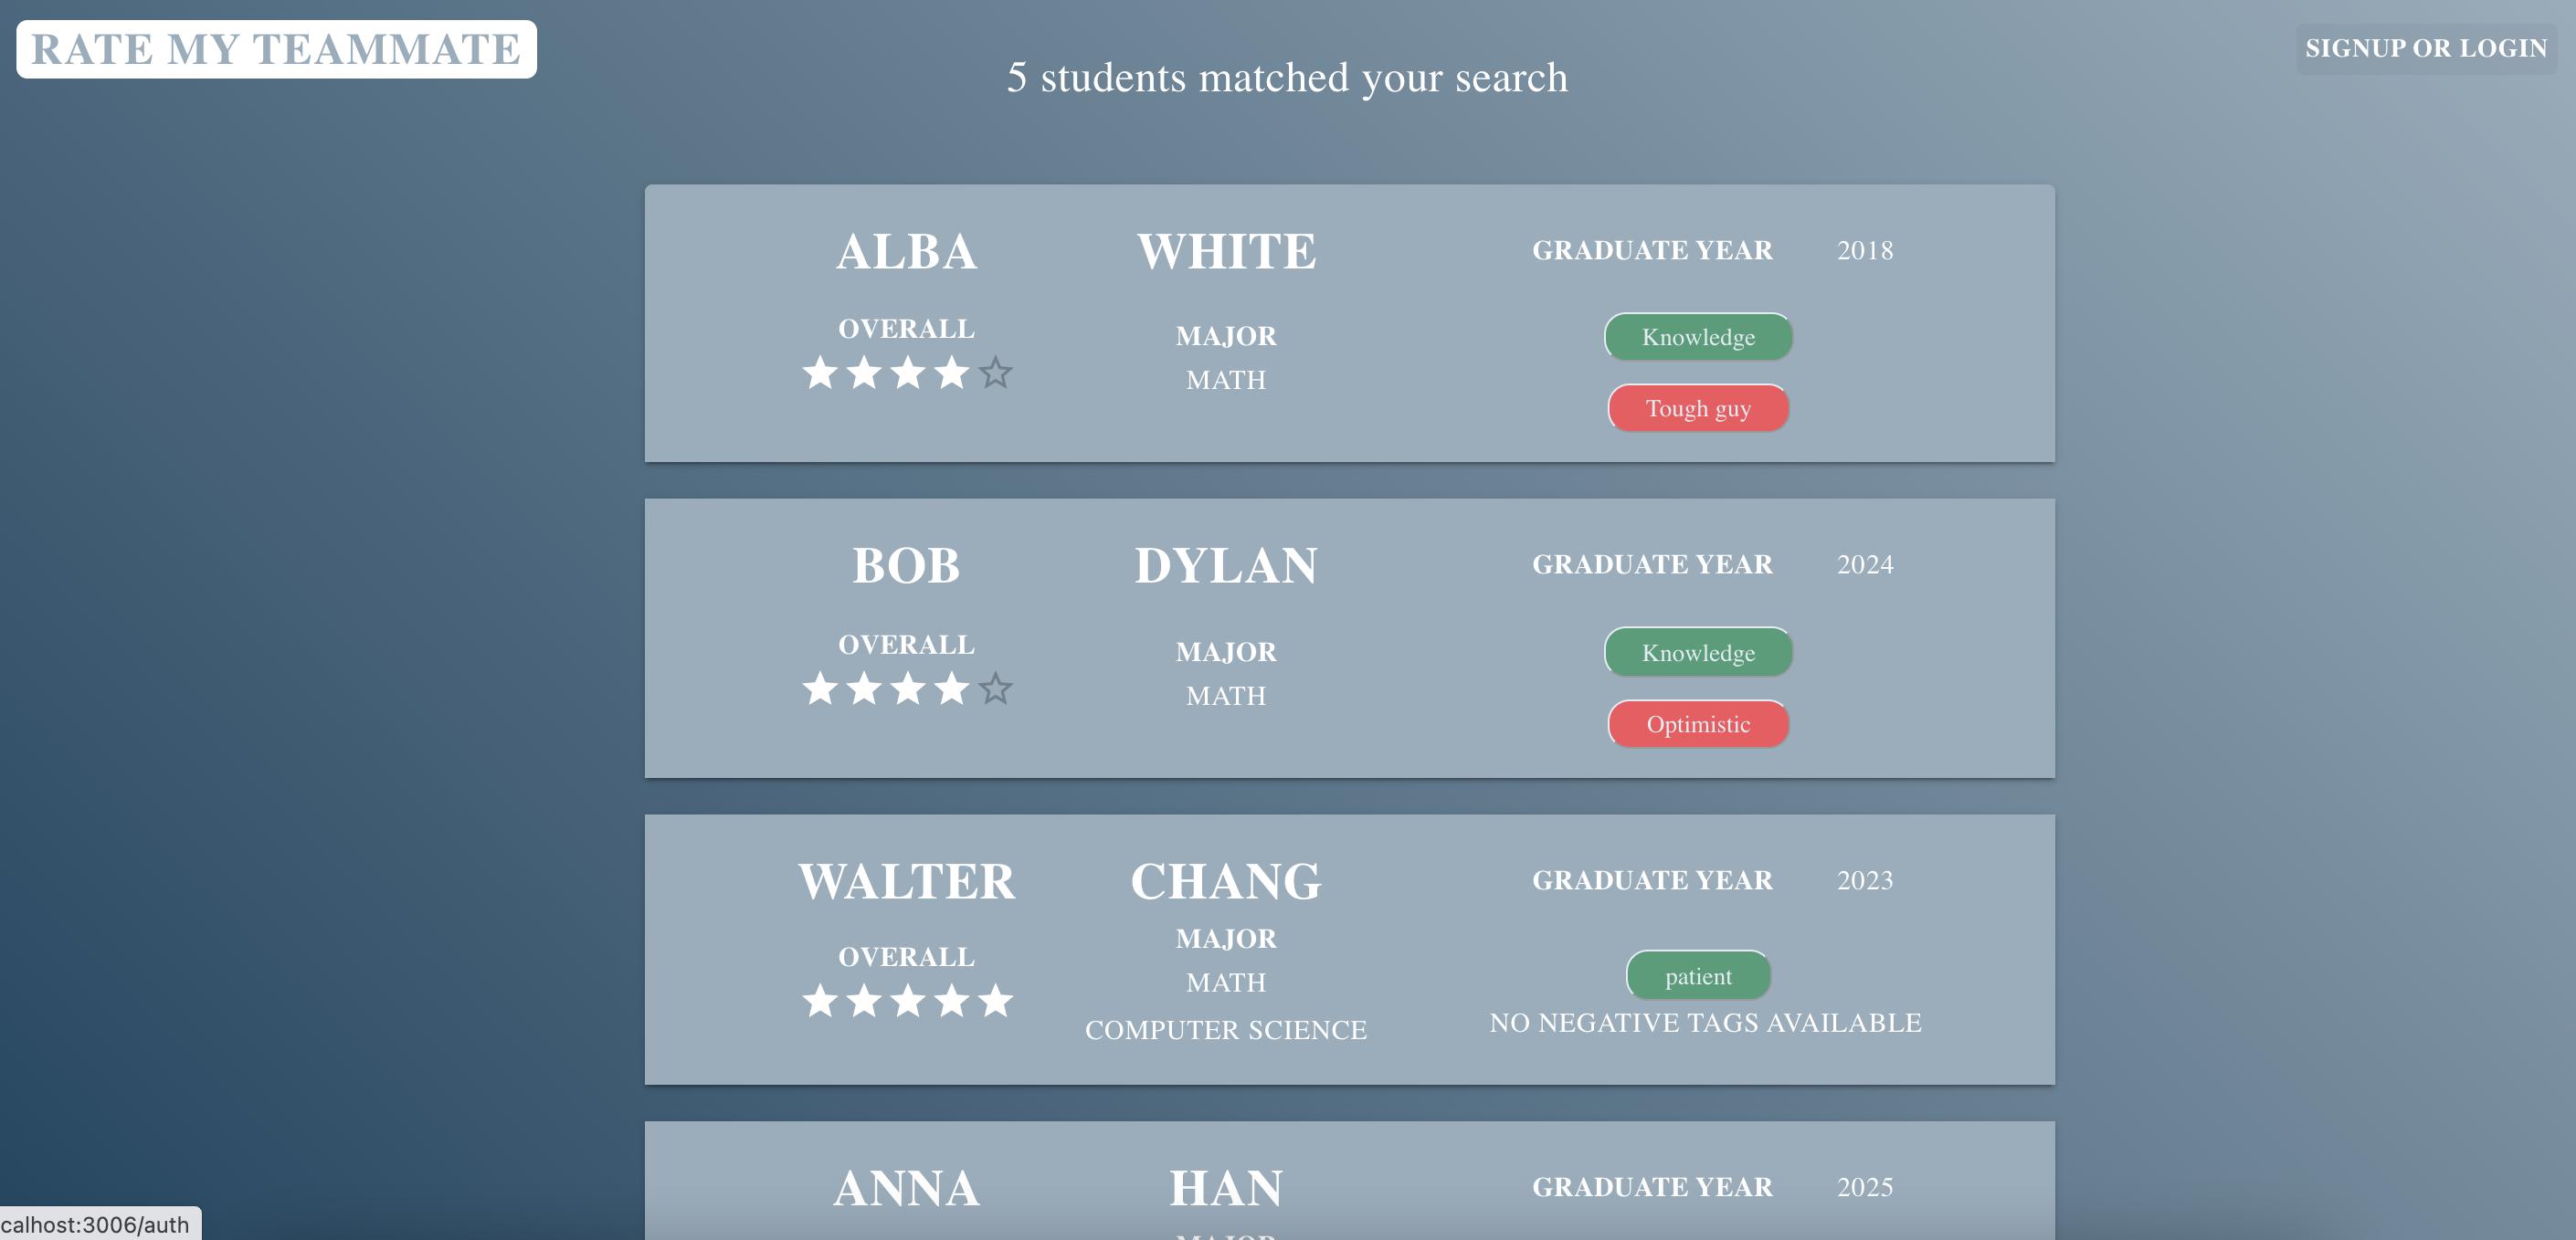
\includegraphics[scale=0.3]{result.png}
    \caption{Result Page of finding students whose major is ``Math''}
    \label{fig:result}
\end{figure}

\begin{figure}[h]
    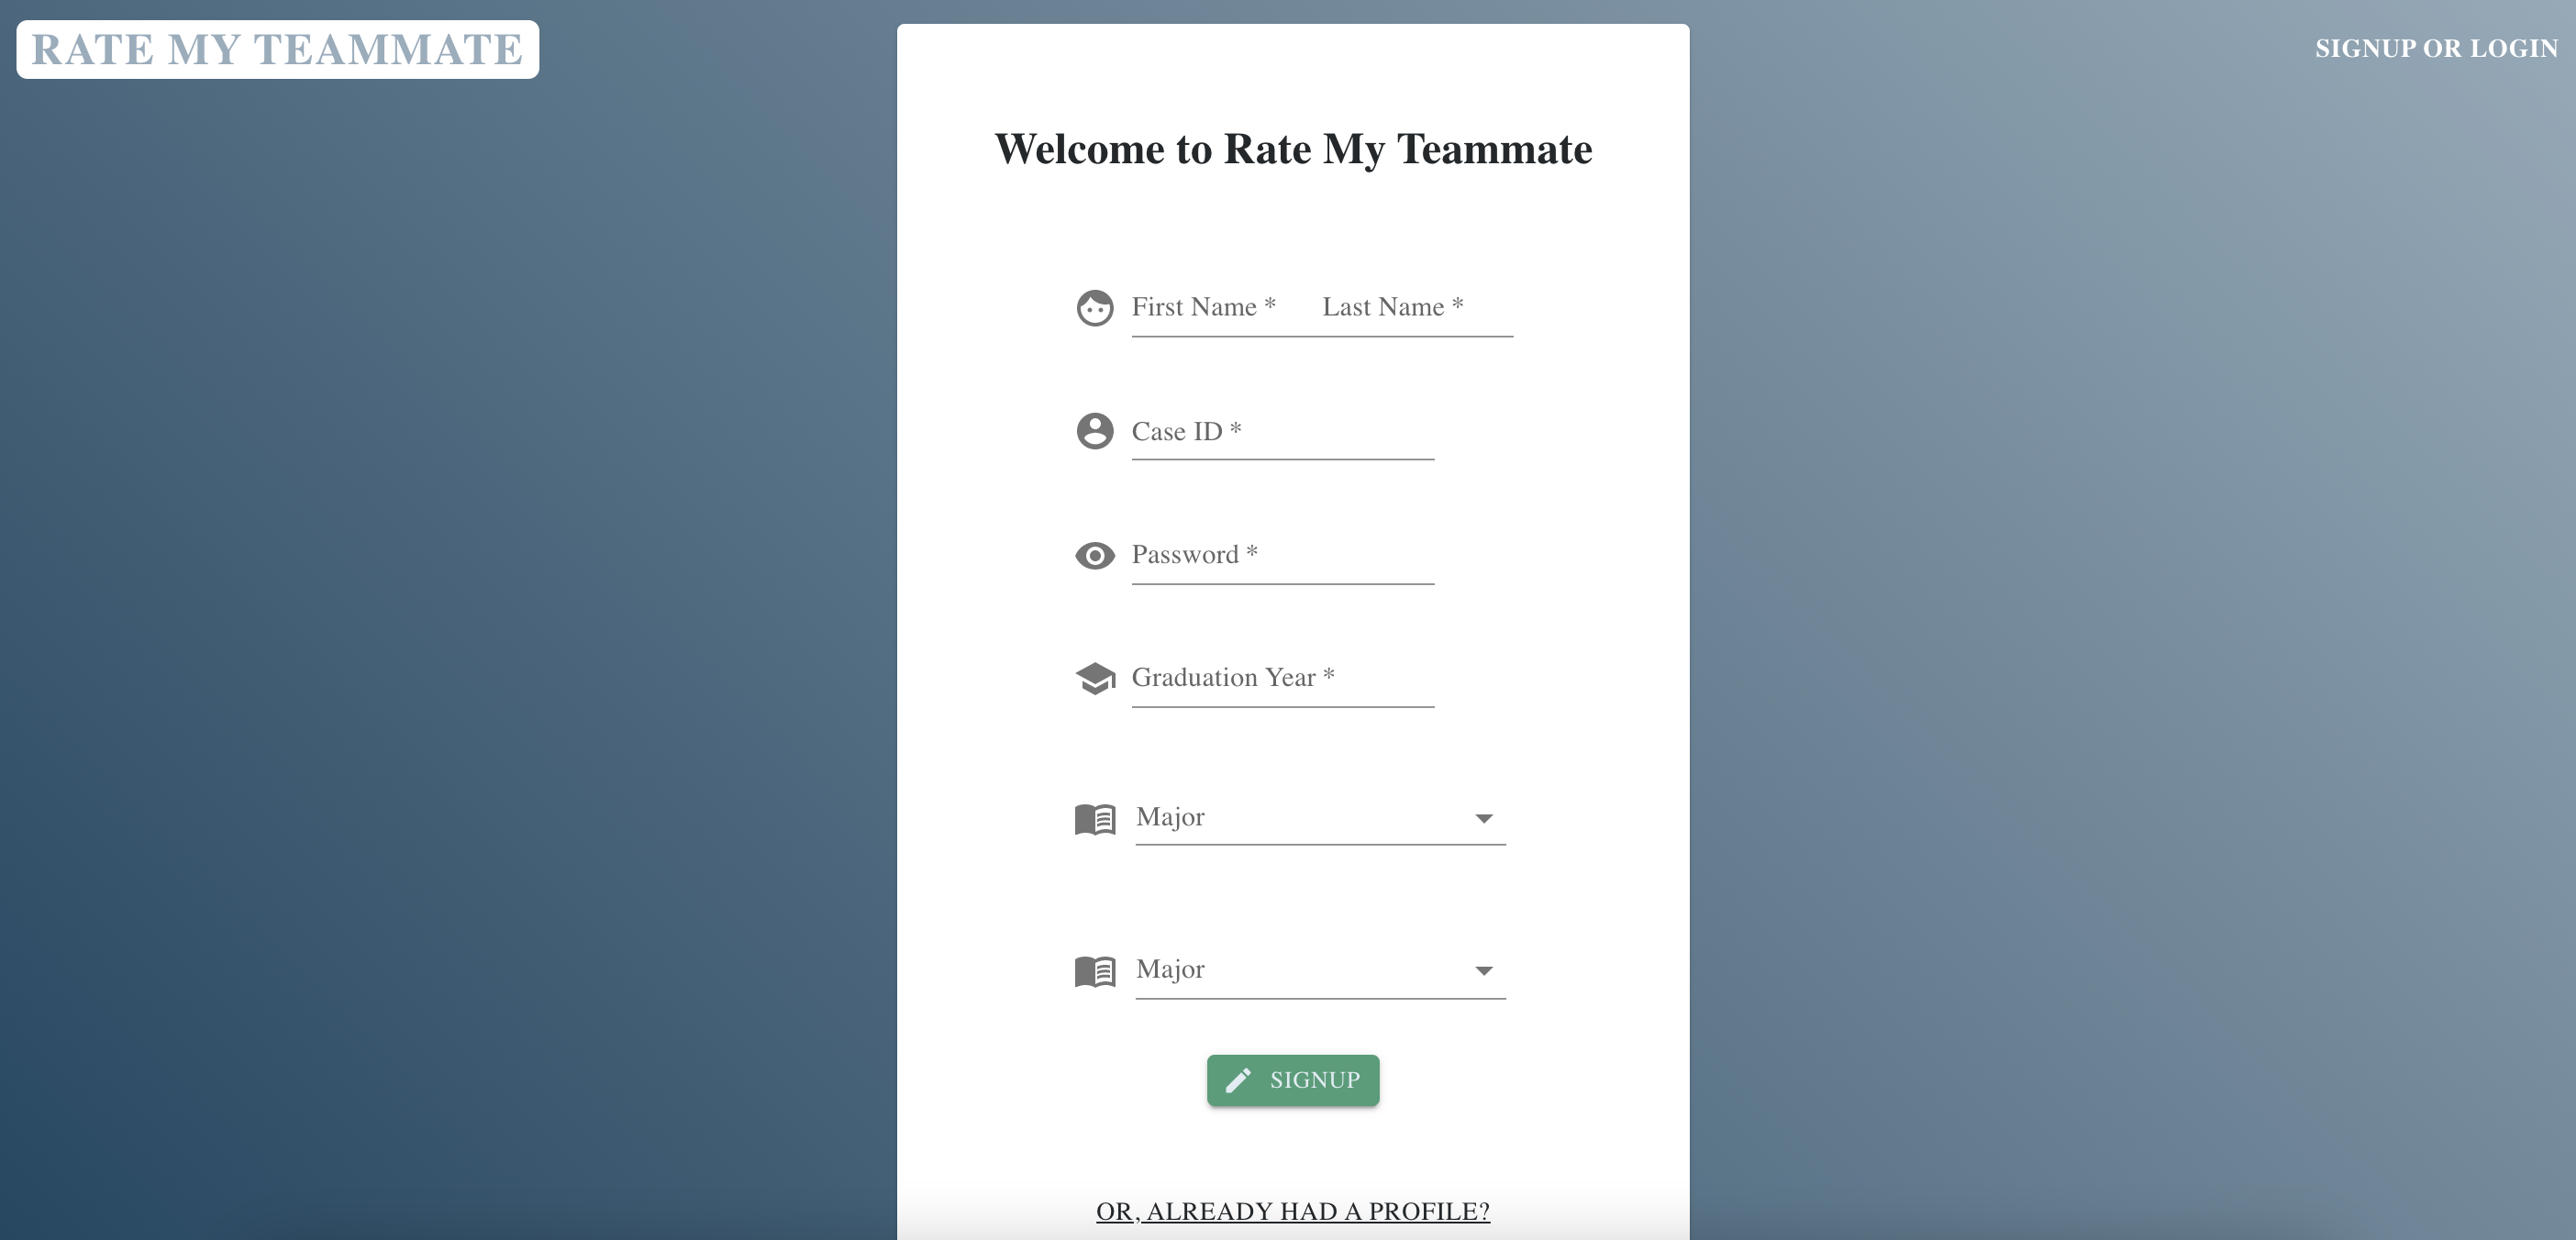
\includegraphics[scale=0.3]{signup.png}
    \caption{Sign up page}
    \label{fig:signup}
\end{figure}
\begin{figure}[h]
    \centering
    
\includegraphics[scale=0.3]{login.png}
    \caption{Login page}
    \label{fig:login}
\end{figure}

\begin{figure}[h]
    \centering
    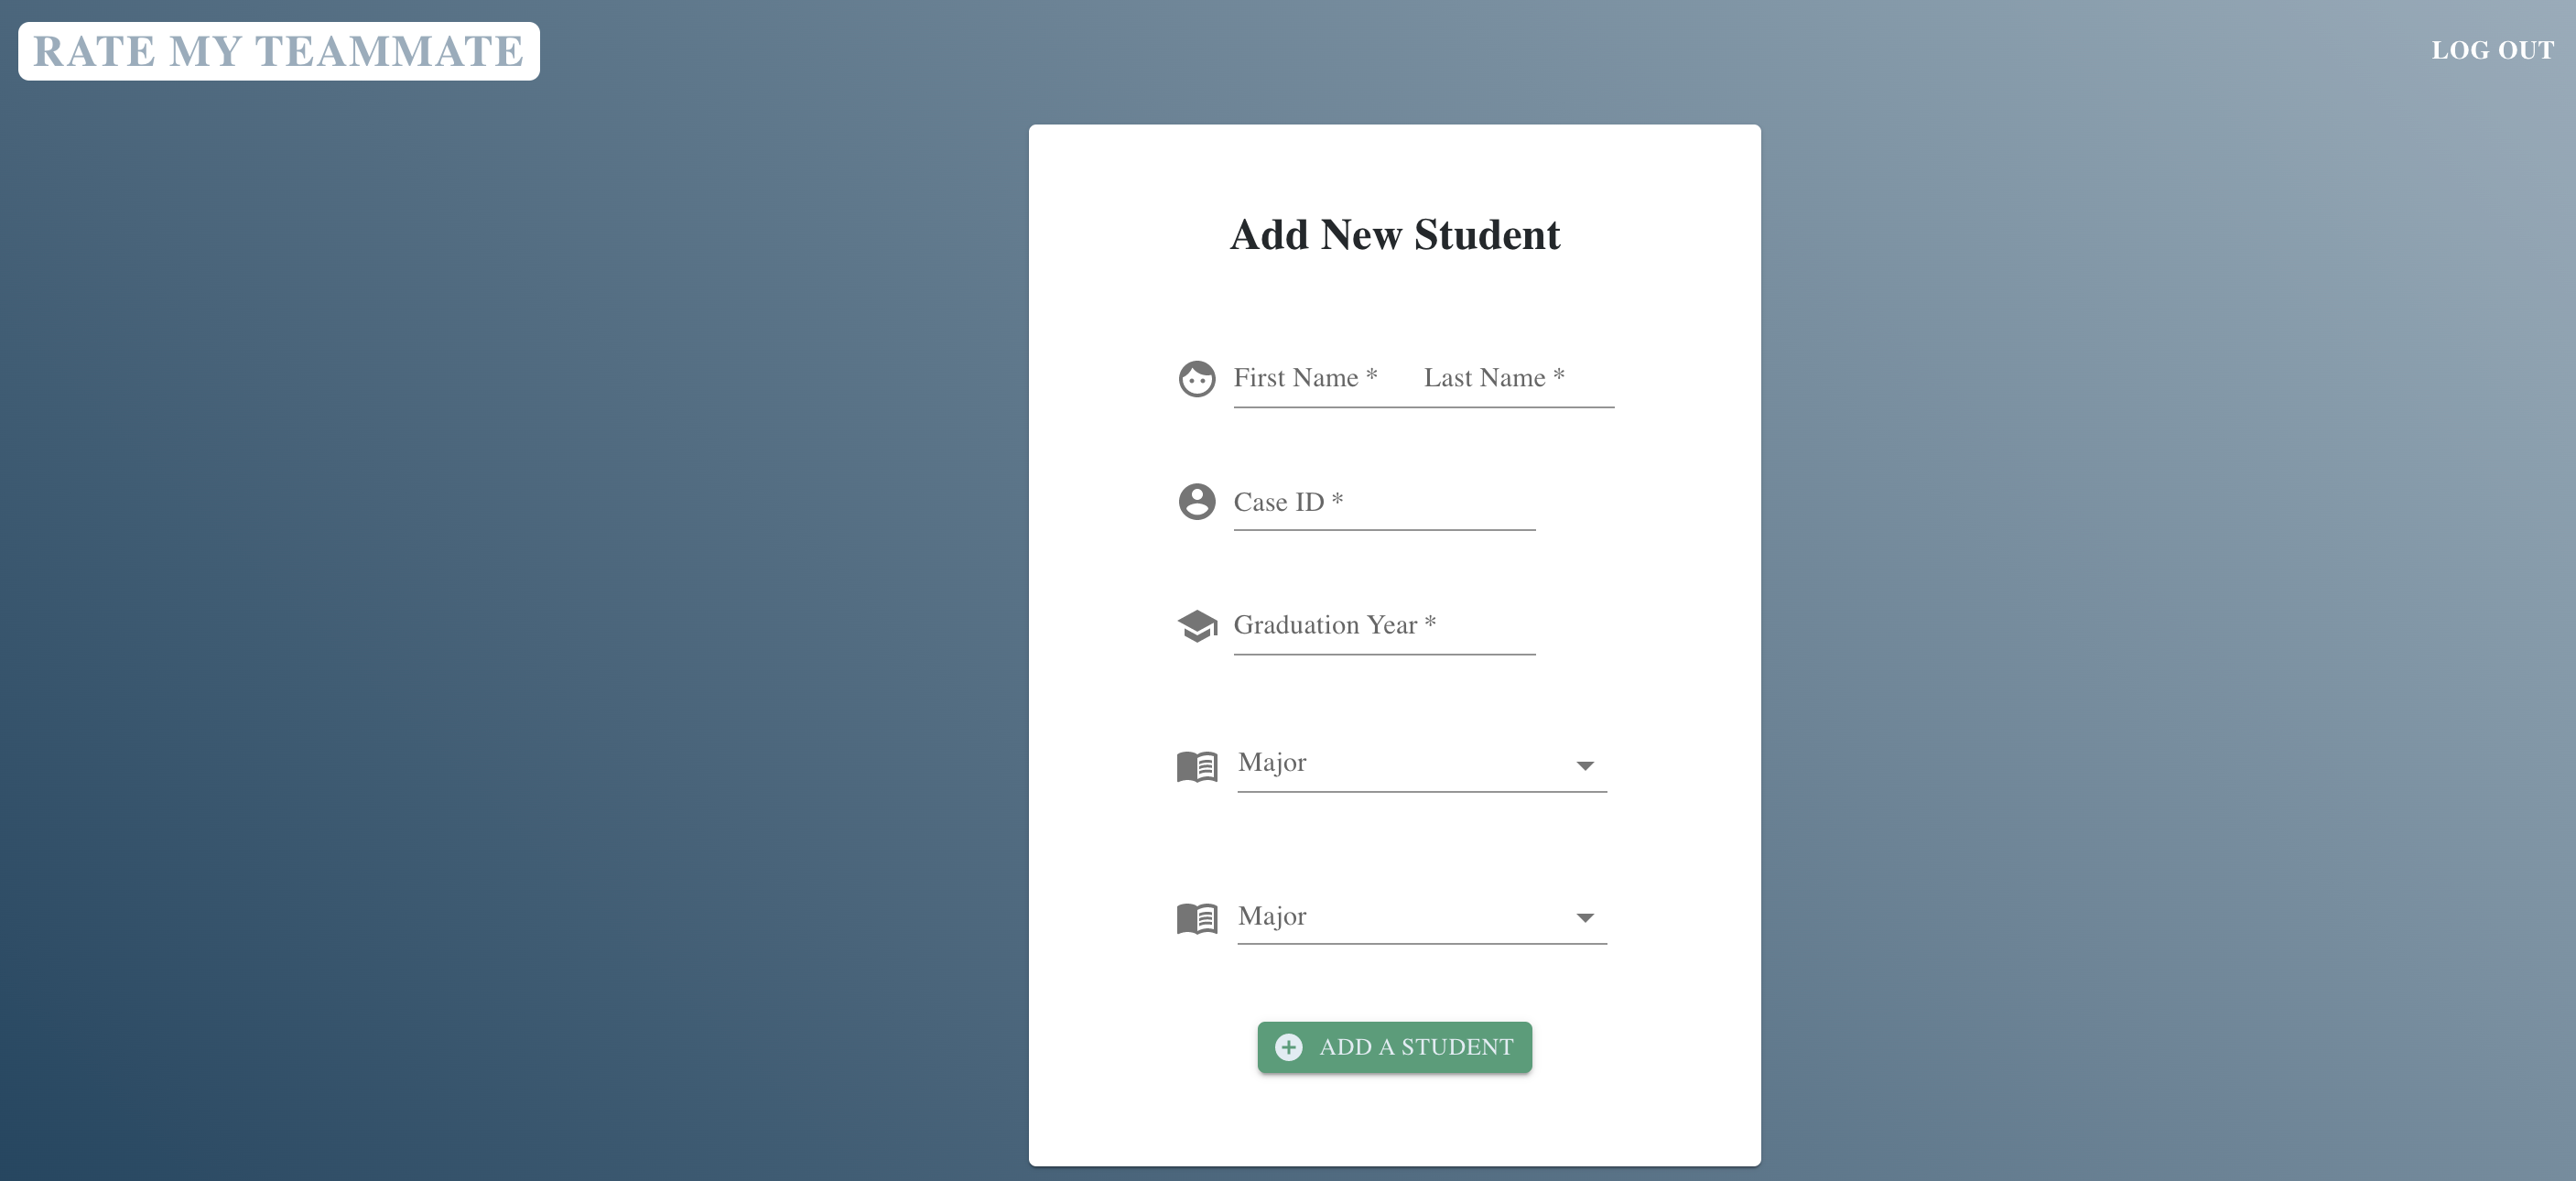
\includegraphics[scale=0.3]{addstudent.png}
    \caption{Add new student page}
    \label{fig:add}
\end{figure}

\begin{figure}[h]
    \centering
    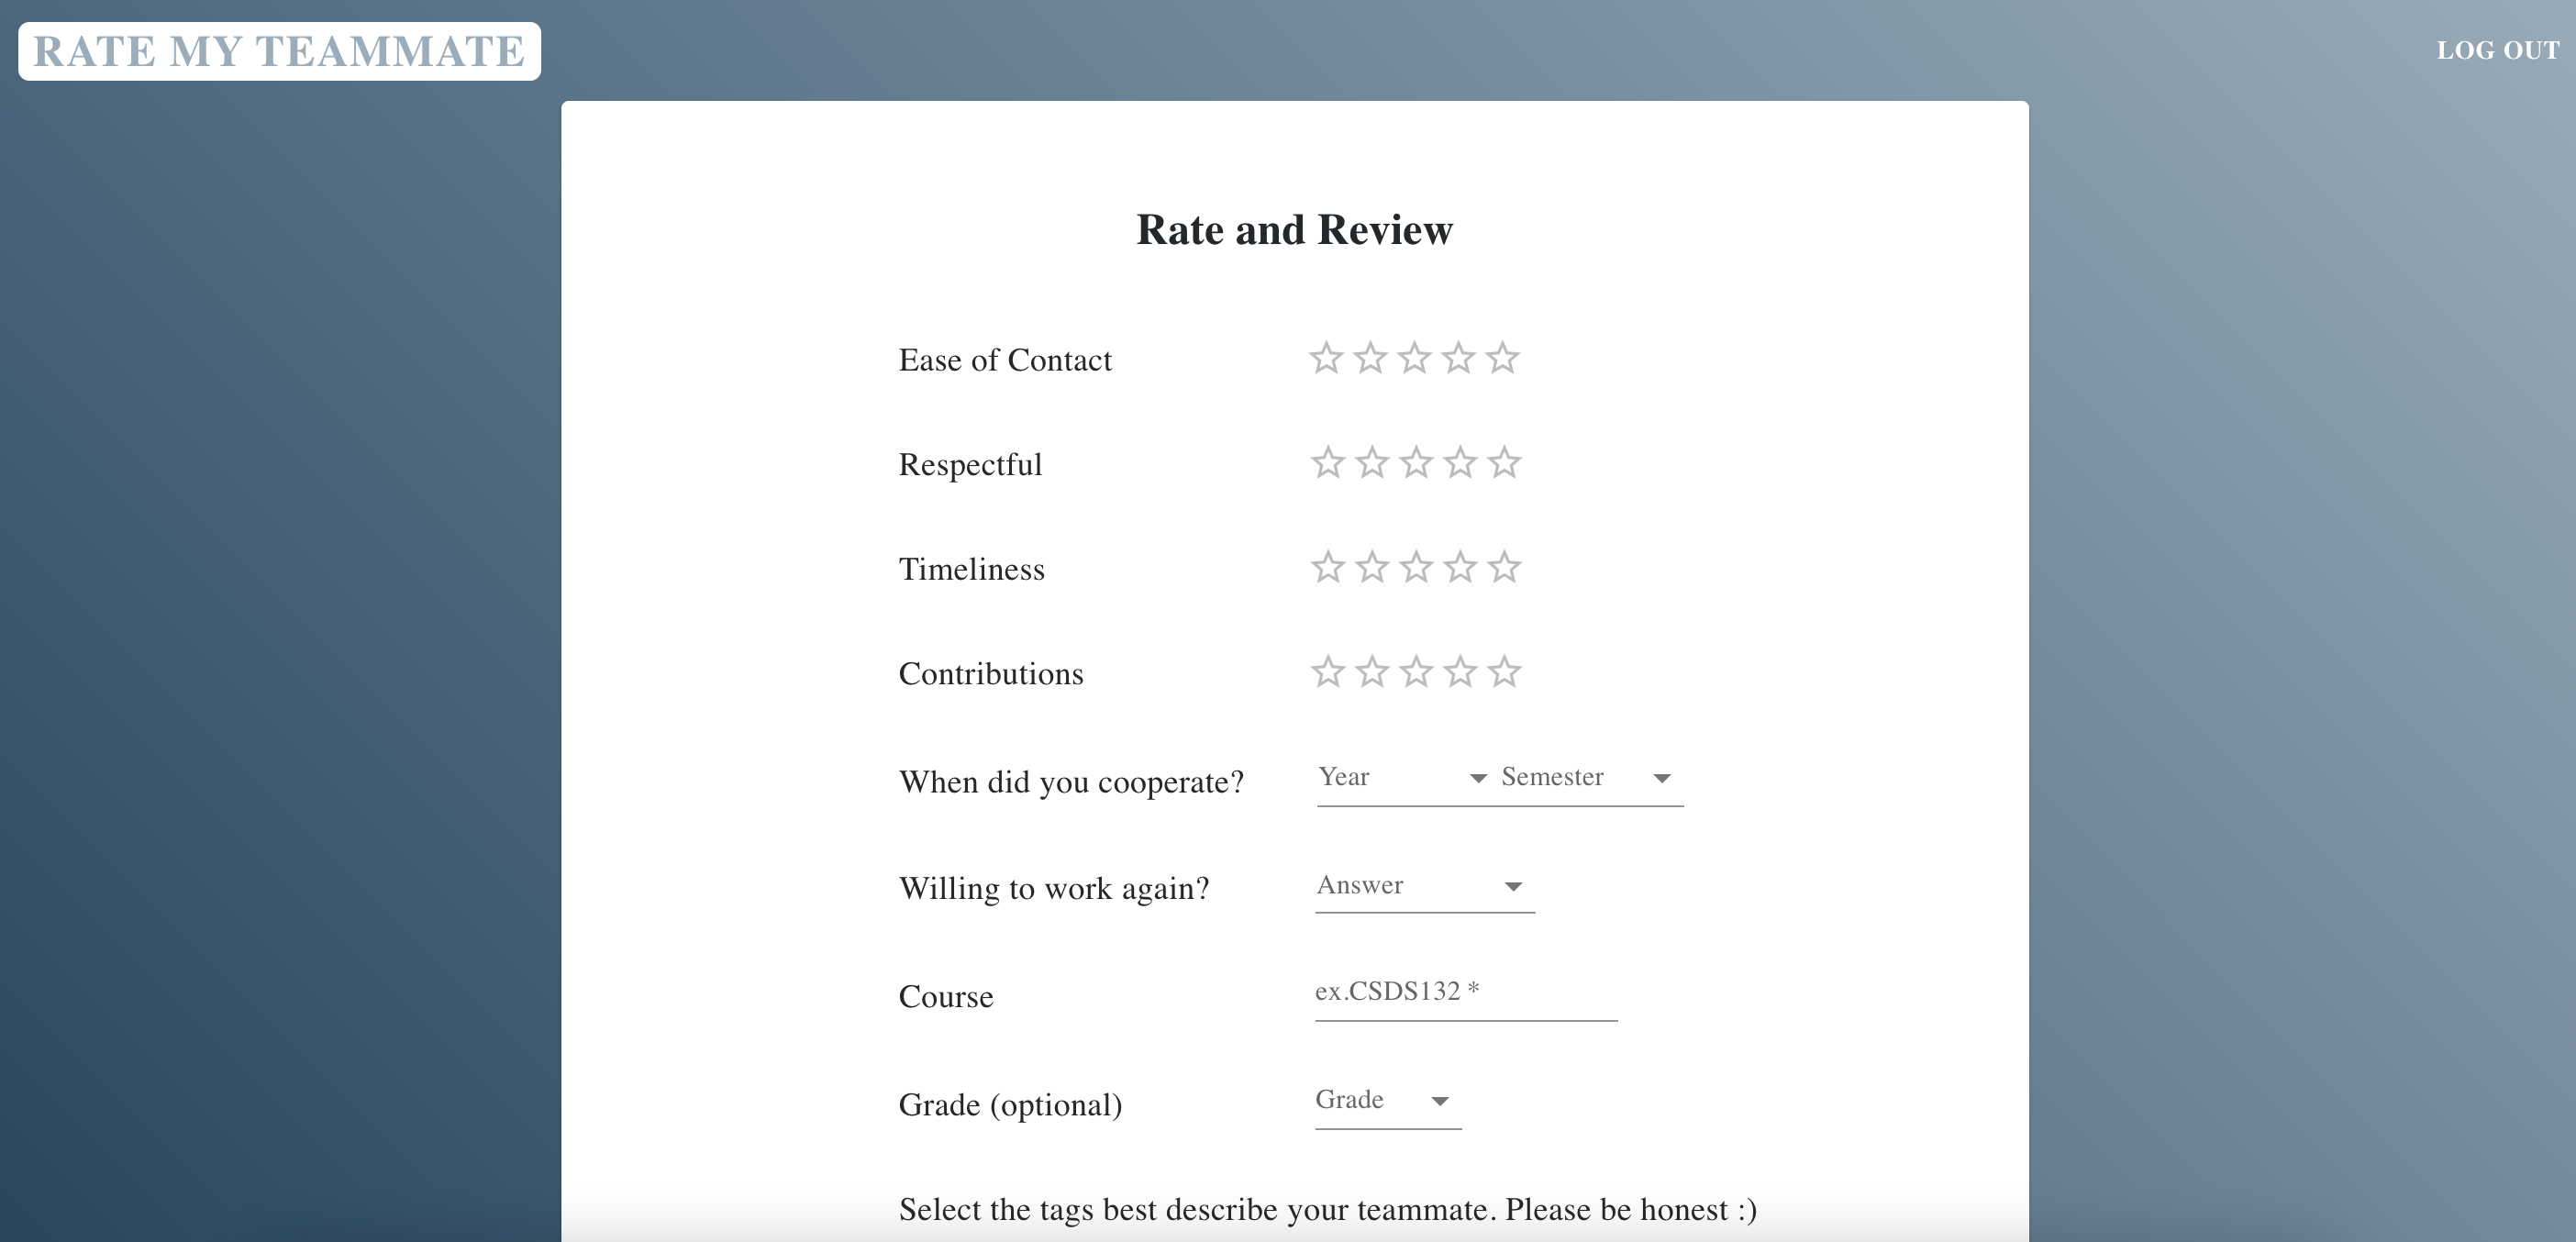
\includegraphics[scale=0.2]{review-up.png}
    \centering
    
\includegraphics[scale=0.2]{review-down.png}
    \caption{Add new review page}
    \label{fig:review}
\end{figure}

\begin{figure}[h]
    \centering
    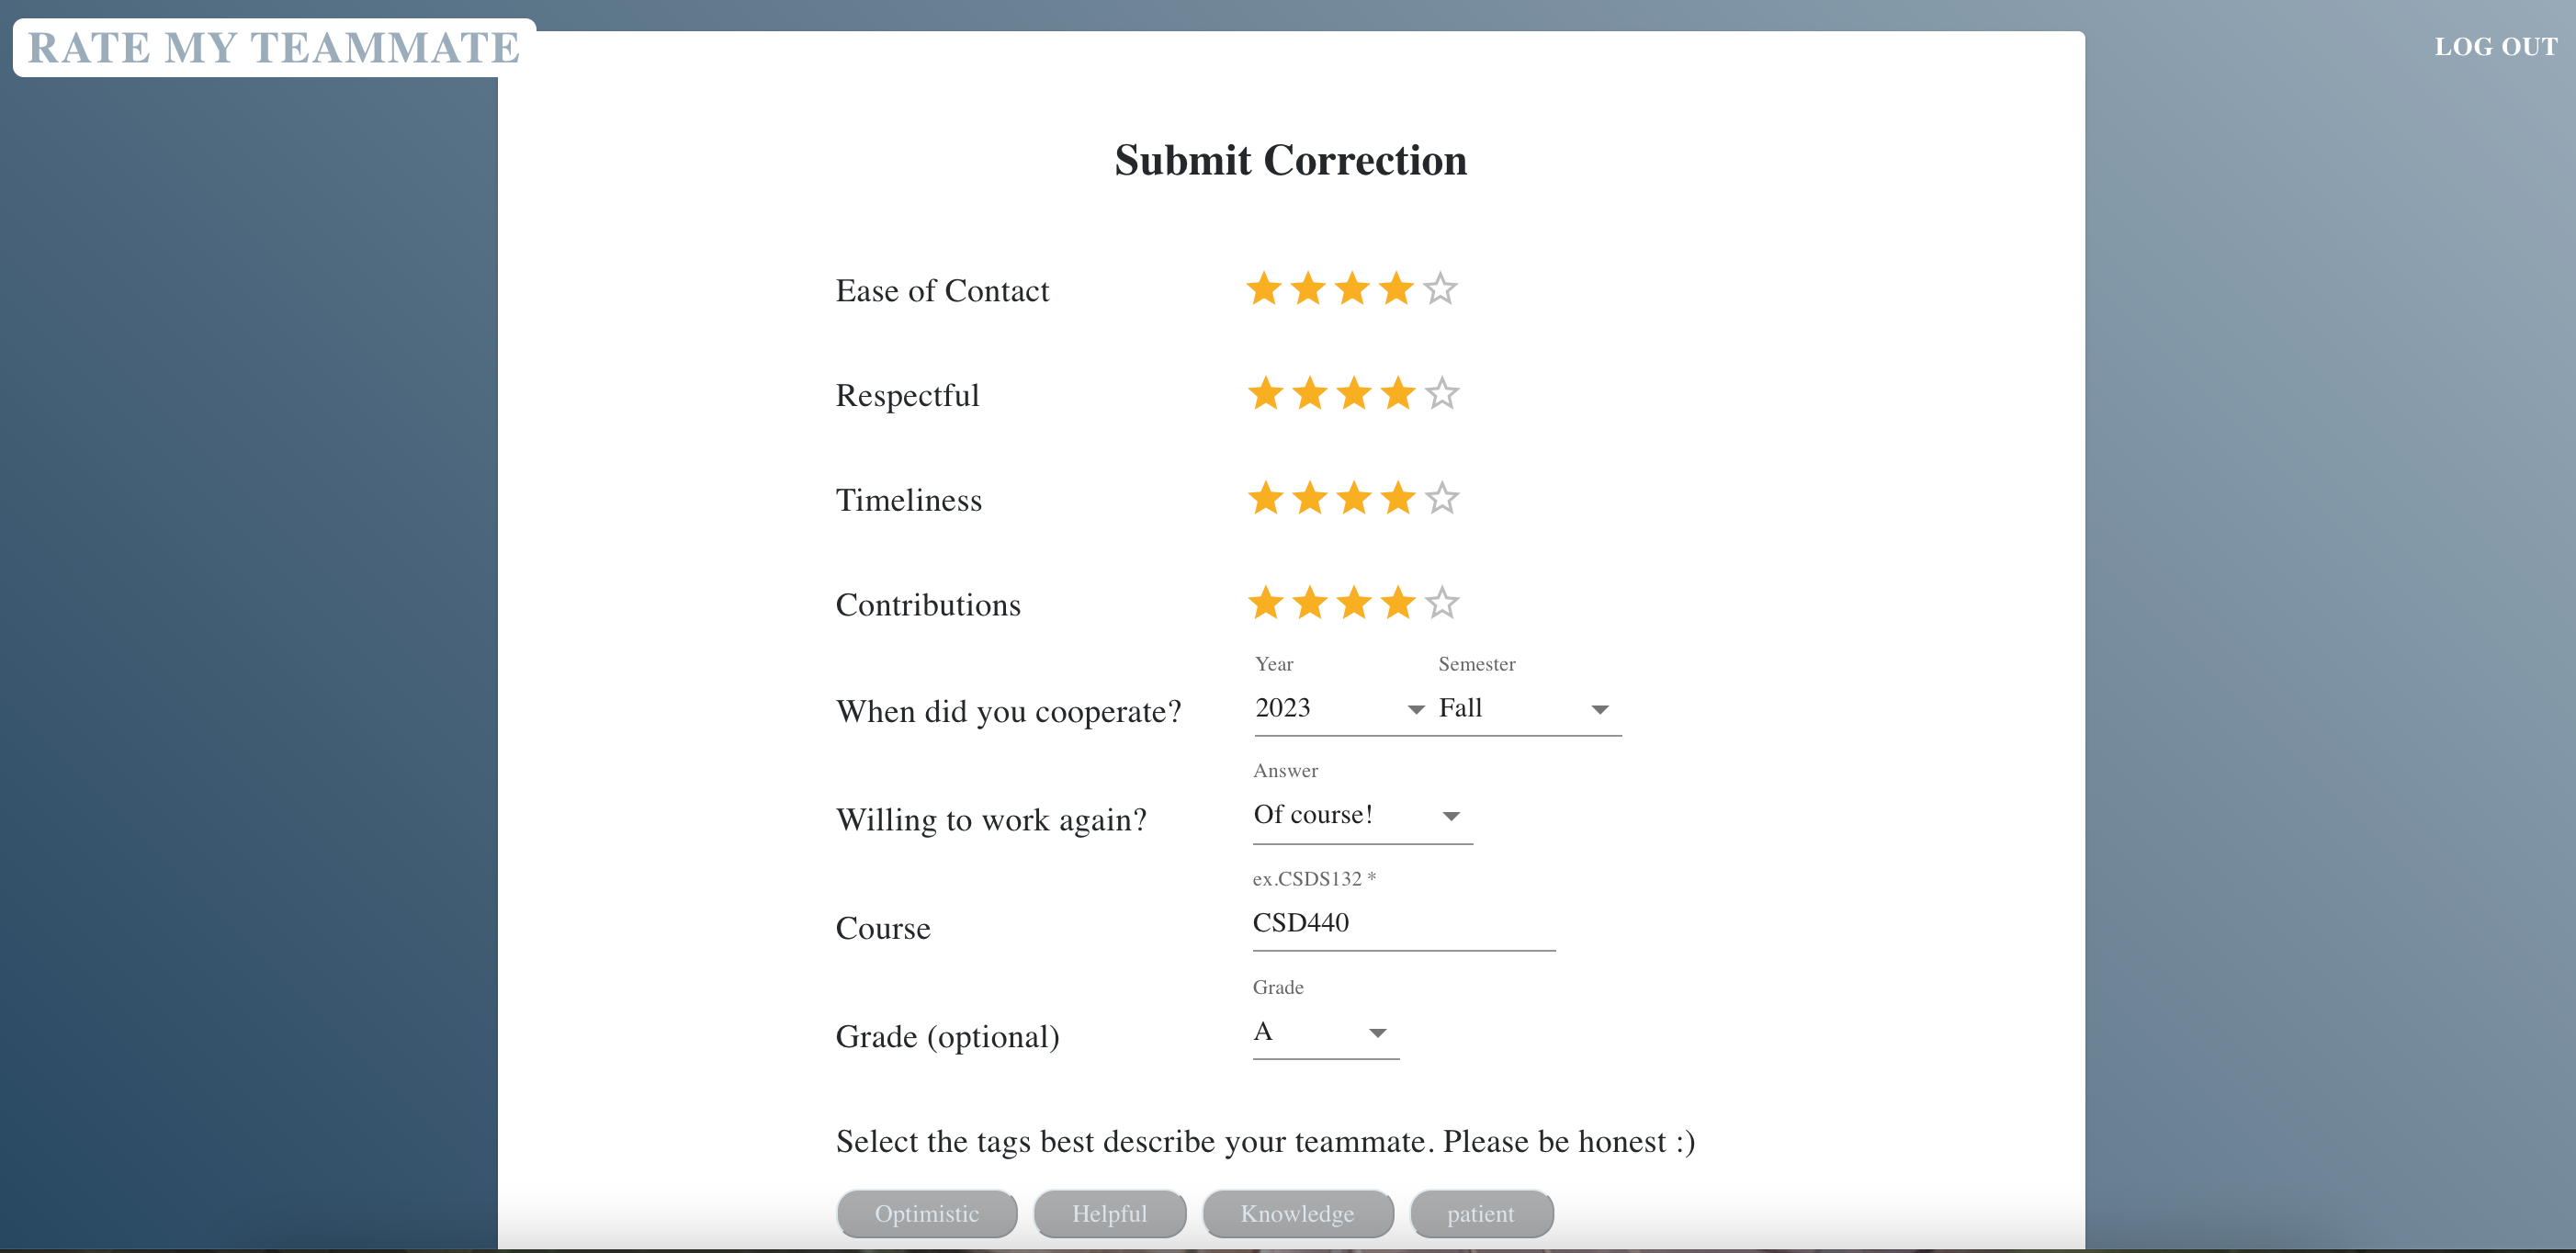
\includegraphics[scale=0.2]{correction-up.png}
    \centering
    
\includegraphics[scale=0.2]{correction-down.png}
    \caption{Submit correction for a certain review}
    \label{fig:correction}
\end{figure}

\begin{figure}[h]
    \centering
    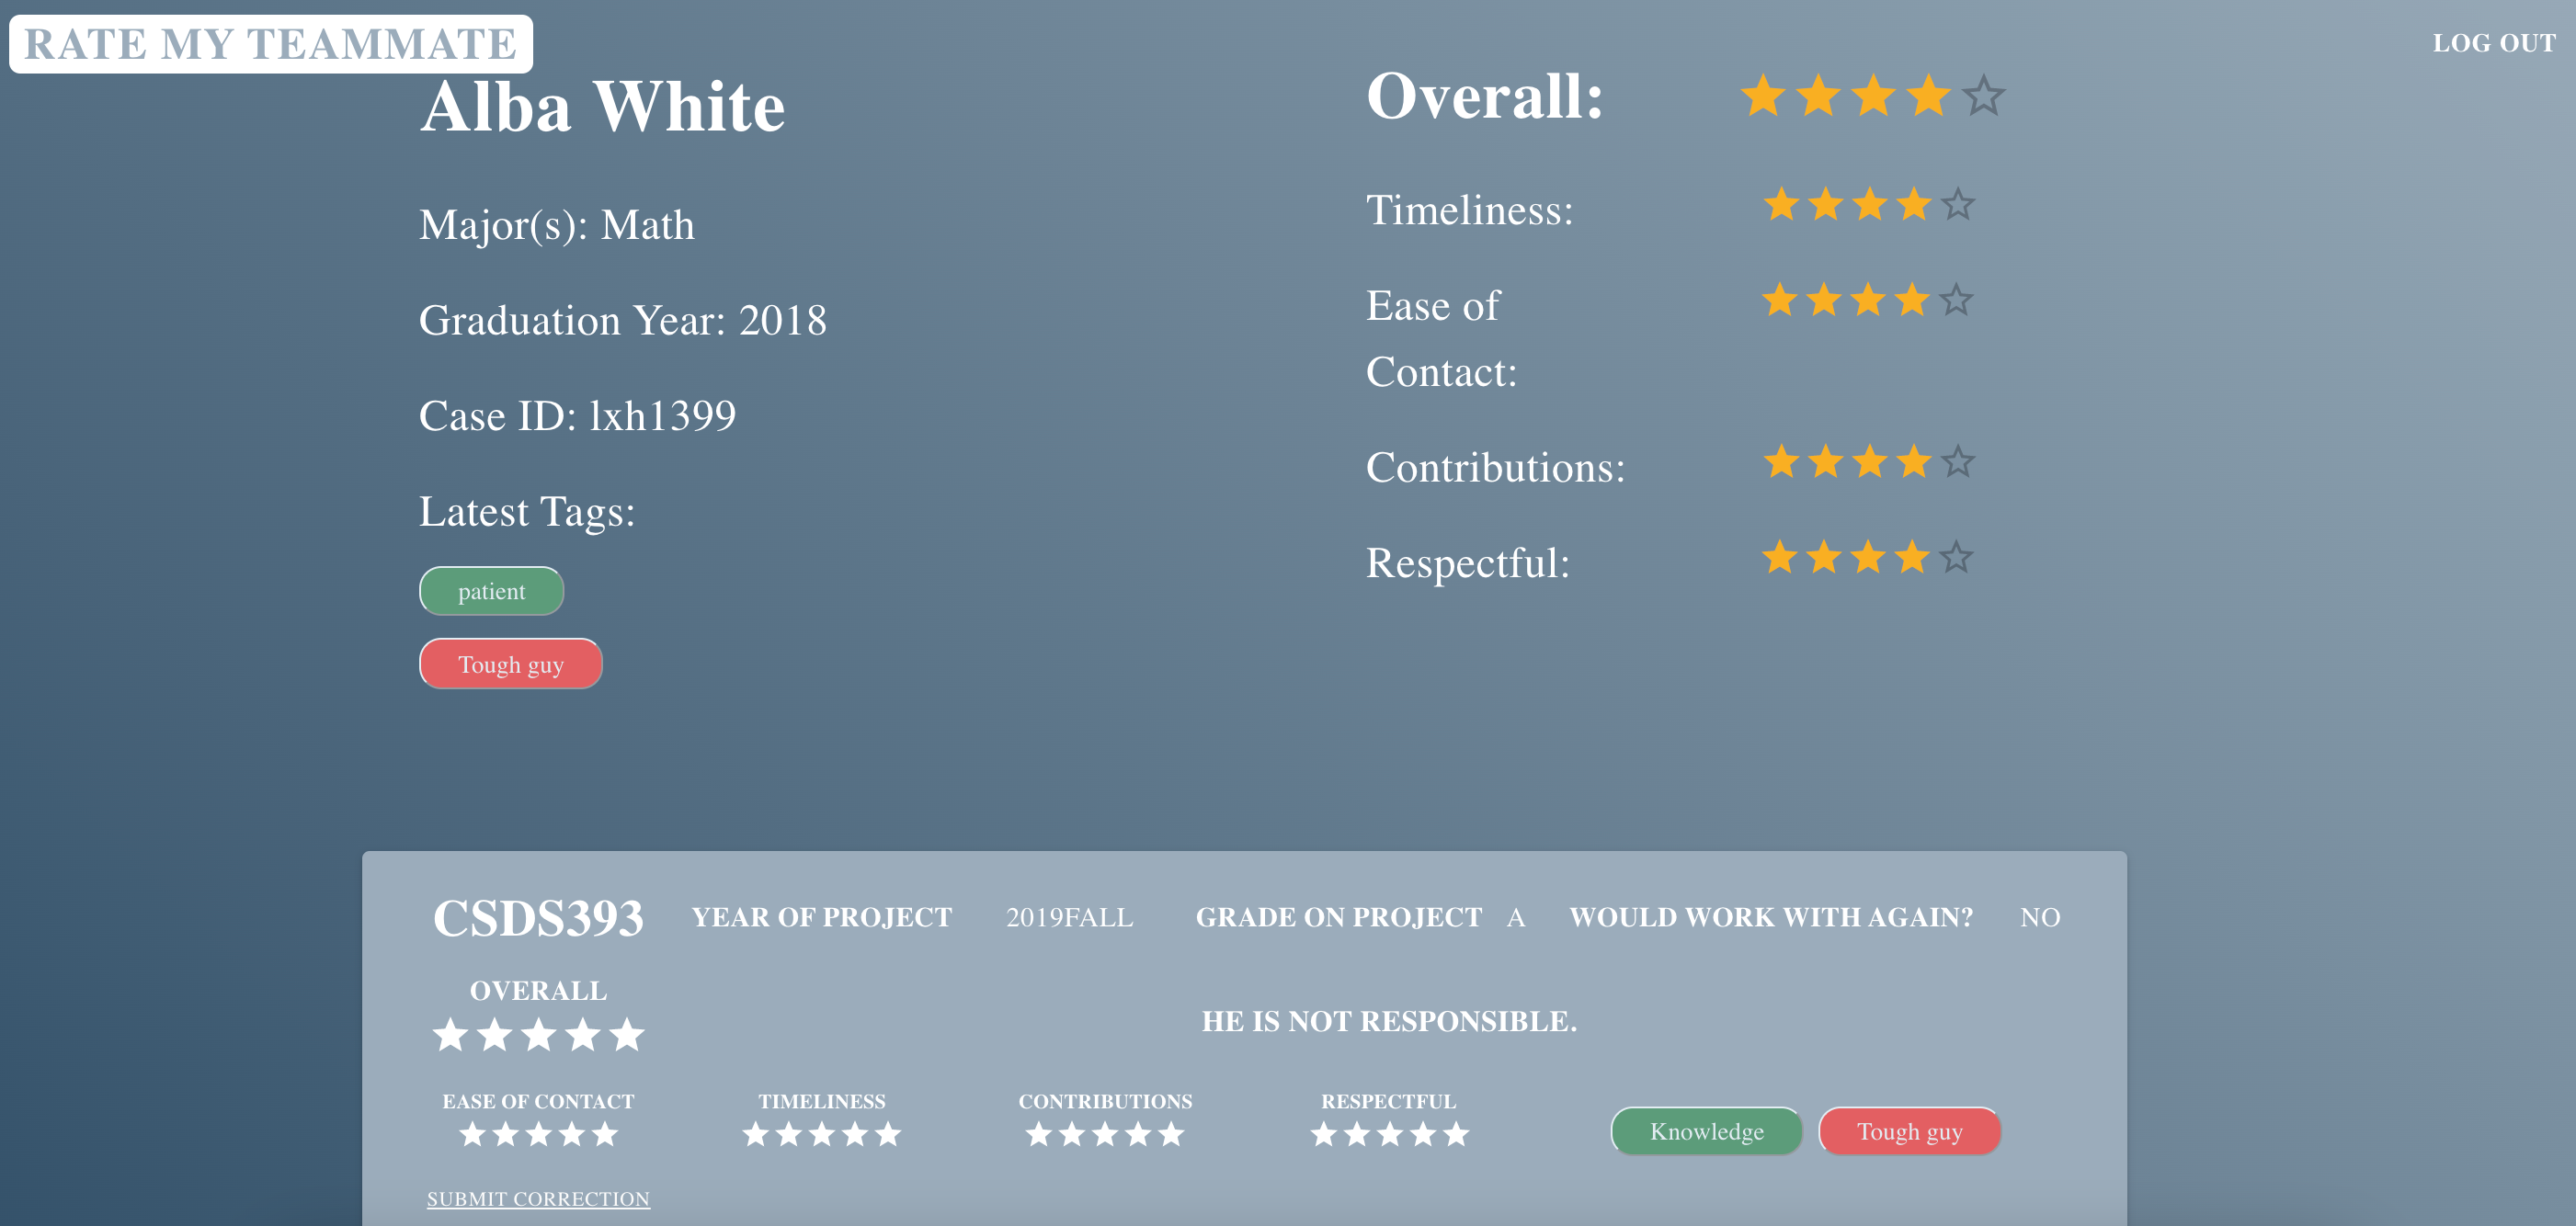
\includegraphics[scale=0.3]{student.png}
    \caption{Sample student information page}
    \label{fig:profile}
\end{figure}

\end{document}
